% inspired from http://tex.stackexchange.com/questions/63612/tikz-tree-drawing-with-comments-to-each-level
\documentclass{article}

\usepackage[utf8]{inputenc}
\usepackage[T1]{fontenc}
\usepackage{tikz}
\usetikzlibrary{arrows}
\usetikzlibrary{shapes, positioning, calc}
\usetikzlibrary{decorations.pathreplacing}

\tikzset{
   treenode/.style = {align = center, inner sep = 0pt, text centered, font = \sffamily}, n/.style = {treenode, circle, font = \sffamily\bfseries, draw, text width = 1.5em}
}

\begin{document}


% 1ère étape : construire le tas à partir du tableau

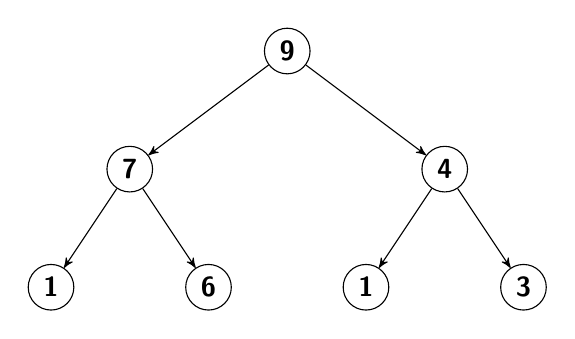
\begin{tikzpicture}[->, >=stealth', level/.style = {sibling distance = 4cm/#1, level distance = 1.5cm}]
   \node [n] {9}
   child{ node [n] {7}
      child{ node [n] {1}
      }
      child{ node [n] {6}
      }                            
   }
   child{ node [n] {4}
      child{ node [n] {1}
      }
      child{ node [n] {3}
      }
   }
   ; 
\end{tikzpicture}

% 2ème étape : parcourir le tas et trier les éléments

\vspace{1cm}

% tour 1

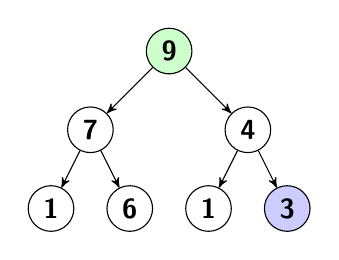
\begin{tikzpicture}[->, >=stealth', level/.style = {sibling distance = 2cm/#1, level distance = 1cm}]
   \node [n, fill = green!20] {9}
   child{ node [n] {7}
      child{ node [n] {1}
      }
      child{ node [n] {6}
      }                            
   }
   child{ node [n] {4}
      child{ node [n] {1}
      }
      child{ node [n, fill = blue!20] {3}
      }
   }
   ; 
\end{tikzpicture}
\hspace{0.5cm}
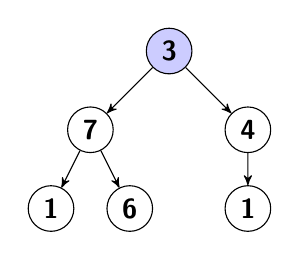
\begin{tikzpicture}[->, >=stealth', level/.style = {sibling distance = 2cm/#1, level distance = 1cm}]
   \node [n,fill = blue!20] {3}
   child{ node [n] {7}
      child{ node [n] {1}
      }
      child{ node [n] {6}
      }                            
   }
   child{ node [n] {4}
      child{ node [n] {1}
      }
   }
   ; 
\end{tikzpicture}
\hspace{0.5cm}
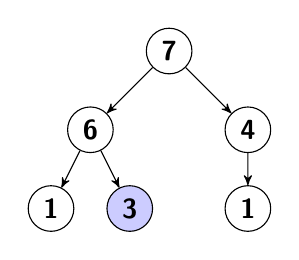
\begin{tikzpicture}[->, >=stealth', level/.style = {sibling distance = 2cm/#1, level distance = 1cm}]
   \node [n] {7}
   child{ node [n] {6}
      child{ node [n] {1}
      }
      child{ node [n, fill = blue!20] {3}
      }                            
   }
   child{ node [n] {4}
      child{ node [n] {1}
      }
   }
   ; 
\end{tikzpicture}

\vspace{0.5cm}
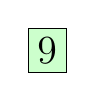
\begin{tikzpicture}
   \node [fill=green!20, font=\sffamily\Large\bfseries, draw, anchor=center] (first) {$9$};
\end{tikzpicture}

% tour 2

\newpage

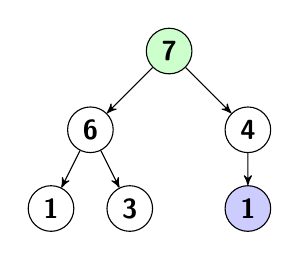
\begin{tikzpicture}[->, >=stealth', level/.style = {sibling distance = 2cm/#1, level distance = 1cm}]
   \node [n, fill = green!20] {7}
   child{ node [n] {6}
      child{ node [n] {1}
      }
      child{ node [n] {3}
      }                            
   }
   child{ node [n] {4}
      child{ node [n, fill = blue!20] {1}
      }
   }
   ; 
\end{tikzpicture}
\hspace{0.5cm}
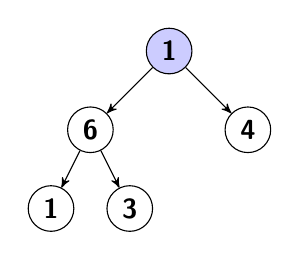
\begin{tikzpicture}[->, >=stealth', level/.style = {sibling distance = 2cm/#1, level distance = 1cm}]
   \node [n, fill = blue!20] {1}
   child{ node [n] {6}
      child{ node [n] {1}
      }
      child{ node [n] {3}
      }                            
   }
   child{ node [n] {4}
   }
   ; 
\end{tikzpicture}
\hspace{0.5cm}
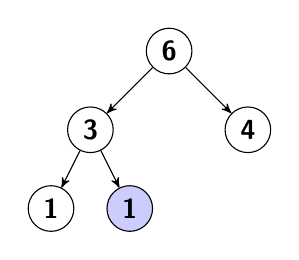
\begin{tikzpicture}[->, >=stealth', level/.style = {sibling distance = 2cm/#1, level distance = 1cm}]
   \node [n] {6}
   child{ node [n] {3}
      child{ node [n] {1}
      }
      child{ node [n, fill = blue!20] {1}
      }                            
   }
   child{ node [n] {4}
   }
   ; 
\end{tikzpicture}

\vspace{0.5cm}
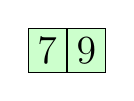
\begin{tikzpicture}
   \node [fill=green!20, font=\sffamily\Large\bfseries, draw, anchor=center] (first) {$7$};
   \node [fill=green!20, font=\sffamily\Large\bfseries, draw, anchor=center, right=0cm of first] (second) {$9$};
\end{tikzpicture}

% tour 3

\vspace{1cm}

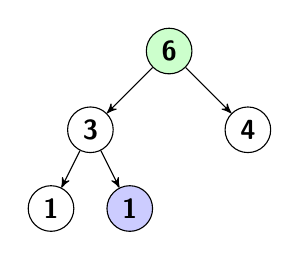
\begin{tikzpicture}[->, >=stealth', level/.style = {sibling distance = 2cm/#1, level distance = 1cm}]
   \node [n, fill = green!20] {6}
   child{ node [n] {3}
      child{ node [n] {1}
      }
      child{ node [n, fill = blue!20] {1}
      }                            
   }
   child{ node [n] {4}
   }
   ; 
\end{tikzpicture}
\hspace{0.5cm}
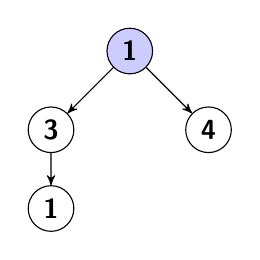
\begin{tikzpicture}[->, >=stealth', level/.style = {sibling distance = 2cm/#1, level distance = 1cm}]
   \node [n, fill = blue!20] {1}
   child{ node [n] {3}
      child{ node [n] {1}
      }                        
   }
   child{ node [n] {4}
   }
   ; 
\end{tikzpicture}
\hspace{0.5cm}
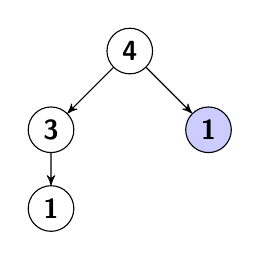
\begin{tikzpicture}[->, >=stealth', level/.style = {sibling distance = 2cm/#1, level distance = 1cm}]
   \node [n] {4}
   child{ node [n] {3}
      child{ node [n] {1}
      }                        
   }
   child{ node [n, fill = blue!20] {1}
   }
   ; 
\end{tikzpicture}

\vspace{0.5cm}
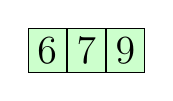
\begin{tikzpicture}
   \node [fill=green!20, font=\sffamily\Large\bfseries, draw, anchor=center] (first) {$6$};
   \node [fill=green!20, font=\sffamily\Large\bfseries, draw, anchor=center, right=0cm of first] (second) {$7$};
   \node [fill=green!20, font=\sffamily\Large\bfseries, draw, anchor=center, right=0cm of second] (third) {$9$};
\end{tikzpicture}

% tour 4

\vspace{1cm}

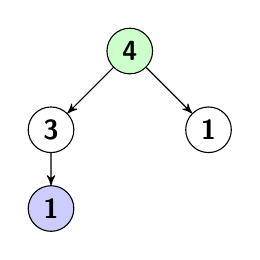
\begin{tikzpicture}[->, >=stealth', level/.style = {sibling distance = 2cm/#1, level distance = 1cm}]
   \node [n, fill = green!20] {4}
   child{ node [n] {3}
      child{ node [n, fill = blue!20] {1}
      }                        
   }
   child{ node [n] {1}
   }
   ; 
\end{tikzpicture}
\hspace{0.5cm}
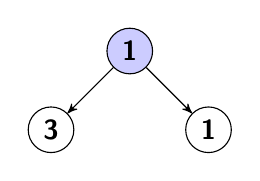
\begin{tikzpicture}[->, >=stealth', level/.style = {sibling distance = 2cm/#1, level distance = 1cm}]
   \node [n, fill = blue!20] {1}
   child{ node [n] {3}           
   }
   child{ node [n] {1}
   }
   ; 
\end{tikzpicture}
\hspace{0.5cm}
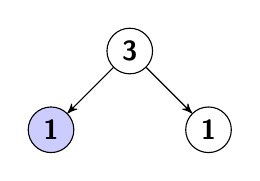
\begin{tikzpicture}[->, >=stealth', level/.style = {sibling distance = 2cm/#1, level distance = 1cm}]
   \node [n] {3}
   child{ node [n, fill = blue!20] {1}           
   }
   child{ node [n] {1}
   }
   ; 
\end{tikzpicture}

\vspace{0.5cm}
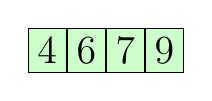
\begin{tikzpicture}
   \node [fill=green!20, font=\sffamily\Large\bfseries, draw, anchor=center] (first) {$4$};
   \node [fill=green!20, font=\sffamily\Large\bfseries, draw, anchor=center, right=0cm of first] (second) {$6$};
   \node [fill=green!20, font=\sffamily\Large\bfseries, draw, anchor=center, right=0cm of second] (third) {$7$};
   \node [fill=green!20, font=\sffamily\Large\bfseries, draw, anchor=center, right=0cm of third] (fourth) {$9$};
\end{tikzpicture}


\vspace{1cm}
...

\vspace{1cm}

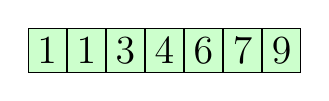
\begin{tikzpicture}
   \node [fill=green!20, font=\sffamily\Large\bfseries, draw, anchor=center] (first) {$1$};
   \node [fill=green!20, font=\sffamily\Large\bfseries, draw, anchor=center, right=0cm of first] (second) {$1$};
   \node [fill=green!20, font=\sffamily\Large\bfseries, draw, anchor=center, right=0cm of second] (third) {$3$};
   \node [fill=green!20, font=\sffamily\Large\bfseries, draw, anchor=center, right=0cm of third] (fourth) {$4$};
   \node [fill=green!20, font=\sffamily\Large\bfseries, draw, anchor=center, right=0cm of fourth] (fifth) {$6$};
   \node [fill=green!20, font=\sffamily\Large\bfseries, draw, anchor=center, right=0cm of fifth] (sixth) {$7$};
   \node [fill=green!20, font=\sffamily\Large\bfseries, draw, anchor=center, right=0cm of sixth] (seventh) {$9$};
\end{tikzpicture}


% Smoothsort : exemple de tas de leonard

\newpage

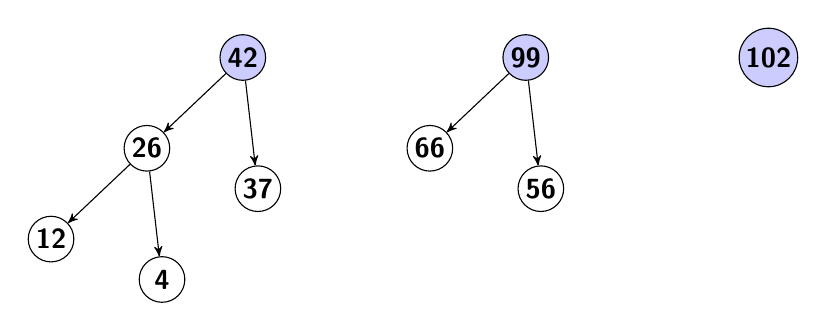
\begin{tikzpicture}[->, >=stealth', grow = 250]
   \node [n, fill=blue!20] (a) {42}
   child{ node [n] {26}
      child{ node [n] {12}
      }
      child{ node [n] {4} }
   }
   child{ node [n] {37} } ; 

   \node [n, fill=blue!20, right=3cm of a] {99}
   child{ node [n] {66} }
   child{ node [n] {56} } ; 

   \node [n, fill=blue!20, text width=2em, right=6cm of a] {102};
\end{tikzpicture}

\end{document}
